下表是六(3)班同学视力情况统计表,请根据表中数据完成下述任务.

\begin{subquestions}

    \subquestion 求该班高度近视同学所占的百分率.

    \subquestion 写出该班视力正常与近视同学的人数比.

    \subquestion 在右图中将该班视力正常,中、轻度近视和高度近视三种同学的人数分别用绿、黄、红三种颜色表示出来,并求出黄色扇形的圆心角的度数.

\end{subquestions}

\begin{center}

    \begin{tabular}{|p{2cm}<{\centering}|p{2cm}<{\centering}|p{3cm}<{\centering}|p{3cm}<{\centering}|}

         \hline

         视力&正常&中、轻度近视&高度近视 \\

         \hline

        人数&18&15&7 \\

        \hline

    \end{tabular}

\end{center}

\begin{center}

    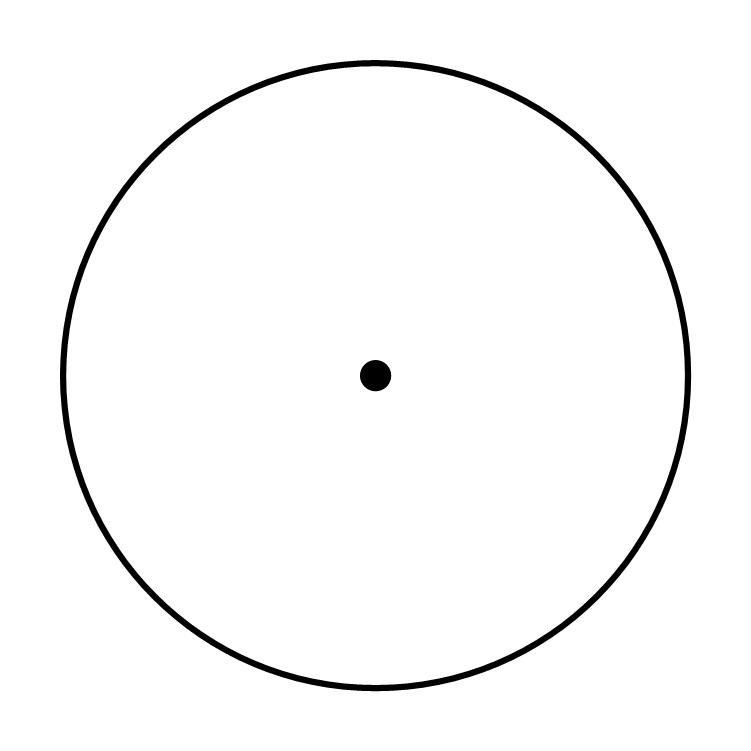
\includegraphics[height=3cm]{lib/image/MJA04040214.png}

\end{center}



